\setcounter{topnumber}{5}
\setcounter{bottomnumber}{5}
\setcounter{totalnumber}{5}

\chapter{Desenvolvimento}
\section{Procedimentos}

\centerline{\begin{minipage}[c]{\textwidth}
		\centering
		\noindent
		\captionof{figure}{Transistor bipolar atuando como fonte de corrente}
		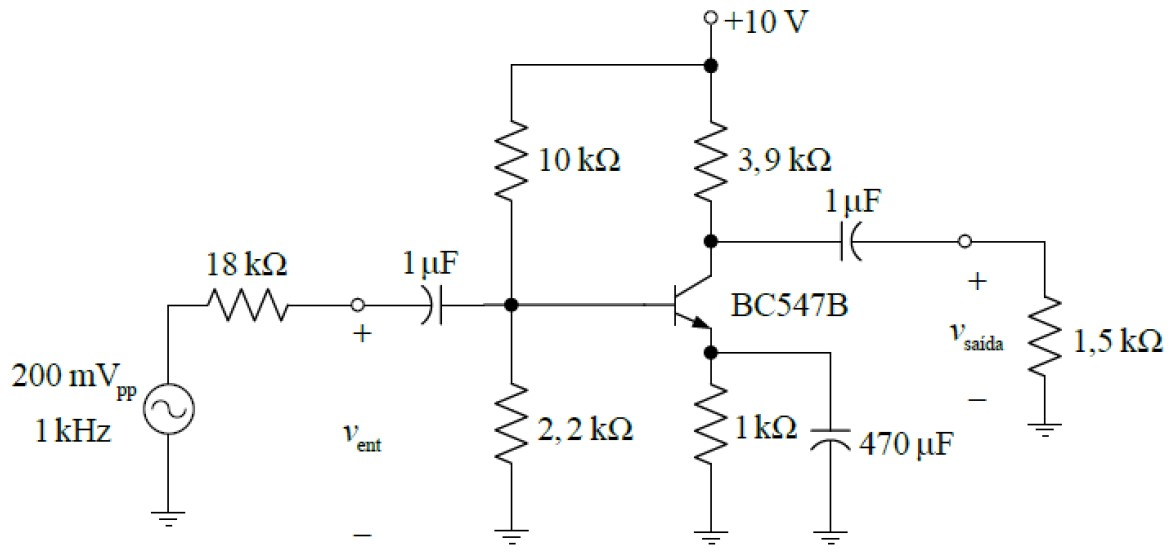
\includegraphics[width=0.9\textwidth]{Imagens/Figura1.jpg}
		\legend{Fonte: Produzido pelos autores}
		\label{Figura1}
\end{minipage}}


\begin{enumerate}
	\item Monte somente o circuito de polarização do circuito da Figura \ref{Figura1}. Com o auxílio do multímetro, meça as variáveis e complete a Tabela \ref{Tabela1}. Caso o seu circuito de polarização esteja operando corretamente, passe para o próximo item desta experiência. Caso  contrário,  descubra  o  que  há  de  errado  com  a  sua  montagem  e  refaça  as  suas medidas $ CC $.
	
	\centerline{\begin{minipage}[c]{\textwidth}
			\centering
			\noindent
			\captionof{table}{Valores $ CC $ teóricos e práticos}
			\begin{tabular}{cccccc}
				\toprule
				Variável & Valor teórico & Valor prático & Erro (\%) \\
				\midrule \midrule
				$V_C$ &   &  &  \\
				\midrule
				$V_B$ &   &  &  \\
				\midrule
				$V_E$ &   &  &  \\
				\midrule
				$V_{CE}$ &   &  &  \\
				\midrule
				$V_{BE}$ &   &  &  \\
				\midrule
				$V_{BC}$ &   &  &  \\
				\midrule
				$I_{C}$ &   &  &  \\
				\midrule
				$I_{B}$ &   &  &  \\
				\midrule
				$I_{E}$ &   &  &  \\
				\midrule
				$\beta_{CC}$ &   &  &  \\
				\midrule
				$P_D$ &   &  &  \\
				\midrule
				\bottomrule
			\end{tabular}%
			\legend{Fonte: Produzido pelos autores}
			\label{Tabela1}
	\end{minipage}}
	
	\item Monte o circuito completo da Figura \ref{Figura1}. Com  o  auxílio  do  osciloscópio,  meça  as variáveis solicitadas e complete a Tabela \ref{Tabela2}. 
	
	
	\centerline{\begin{minipage}[c]{\textwidth}
			\centering
			\noindent
			\captionof{table}{Valores $ CA $ teóricos e práticos}
			\begin{tabular}{cccccc}
				\toprule
				Variável & Valor teórico & Valor prático & Erro (\%) \\
				\midrule \midrule
				$V_{ent}$ &  &  &  \\
				\midrule
				$V_{saída}$ (sem carga) &  &  &  \\
				\midrule
				$V_{saída}$ (com carga) &  &  &  \\
				\midrule
				$A_V$ &  &  &  \\
				\midrule
				$ A_{VC} $ &  &  &  \\
				\midrule
				\bottomrule
			\end{tabular}%
			\legend{Fonte: Produzido pelos autores}
			\label{Tabela2}
	\end{minipage}}
	
	\item Utilize o canal $ 1 $ do osciloscópio para verificar o sinal de entrada do amplificador de tensão e o canal $ 2 $, para o sinal de saída do circuito. Tais formas de onda estão invertidas uma em relação à outra? Por quê?
	
	\item Com o osciloscópio em $ DC $, meça o sinal no coletor do transistor bipolar. Perceba a existência de um nível $ CC $ e de um sinal $ CA $ nesse ponto. Em seguida, verifique o sinal na  carga,  após  o  capacitor  de  $ 1\mu F $.  Note  que  há  apenas  um  sinal  $ CA $.  Por  que  isso ocorre? 
	
	\item Com o osciloscópio em $ DC $, meça o sinal no emissor do transistor bipolar. Perceba a existência de um nível $ CC $. Por que isso ocorre? 
	
	\item Calcule os erros das suas medidas e complete as Tabelas \ref{Tabela1} e \ref{Tabela2}. Considere que o erro é dado por 

$$\%\; de\; erro = \frac{valor \; prático - valor \; teórico}{valor \; teórico} \times 100$$

	\item Analise os seus resultados (valores obtidos, erros, possíveis fonte de erros, ...)

	
	
\end{enumerate}

\section{Resultados}


\centerline{\begin{minipage}[c]{\textwidth}
		\centering
		\noindent
		\captionof{table}{Valores $ CC $ teóricos e práticos}
		\begin{tabular}{cccccc}
			\toprule
			Variável & Valor teórico & Valor prático & Erro (\%) \\
			\midrule \midrule
			$V_C$ &  $ 3,02V $ & $ 5,32V $ & $1,5 \% $ \\
			\midrule
			$V_B$ &  $ 0,7V $ & $ 0,67V $ & $1,5 \% $ \\
			\midrule
			$V_E$ &  $ 0V $ & $ 0,015V $ & $1,5 \% $ \\
			\midrule
			$V_{CE}$ &  $ 3,02V $ & $ 5,32 V $ & $1,5 \% $ \\
			\midrule
			$V_{BE}$ &  $ 3,02V $ & $ 5,32 V $ & $1,5 \% $ \\
			\midrule
			$V_{BC}$ &  $ 3,02V $ & $ 5,32 V $ & $1,5 \% $ \\
			\midrule
			$I_{C}$ &  $ 10,26mA$ & $ 6,87 mA $ & $ 699 \% $ \\
			\midrule
			$I_{B}$ &  $ 34,44\mu A $ & $ 34,44\mu A $ & $ 1,55\% $ \\
			\midrule
			$I_{E}$ &  $ 10,26mA$ & $ 6,87 mA $ & $ 699 \% $ \\
			\midrule
			$\beta_{CC}$ & $ 298 $ & $ 298 $ & $ 87,68 \% $ \\
			\midrule
			$P_D$ &  $ 30,98 mW $ & $ 36,54mW $ & $ \% $ \\
			\midrule
			\bottomrule
		\end{tabular}%
		\legend{Fonte: Produzido pelos autores}
		\label{Tabela3}
\end{minipage}}


\centerline{\begin{minipage}[c]{\textwidth}
		\centering
		\noindent
		\captionof{table}{Valores $ CA $ teóricos e práticos}
		\begin{tabular}{cccccc}
			\toprule
			Variável & Valor teórico & Valor prático & Erro (\%) \\
			\midrule \midrule
			$V_{ent}$ &  $ 20mA $ & $ 19,7 mA $ & $1,5 \% $ \\
			\midrule
			$V_{saída}$ (sem carga) &  $ 1,027mA$ & $ 1,066 mA $ & $ 3,8 \% $ \\
			\midrule
			$V_{saída}$ (com carga) &  $ 20mA $ & $ 19,69 mA $ & $ 1,55 \% $ \\
			\midrule
			$A_V$ &  $ 2,48 V $ & $ 2,449 V $ &  $ 1,25 \% $ \\
			\midrule
			$ A_{VC} $ & $ 18,47 $ & $ 18,47 $ & $ 0\% $ \\
			\midrule
			\bottomrule
		\end{tabular}%
		\legend{Fonte: Produzido pelos autores}
		\label{Tabela4}
\end{minipage}}